\documentclass{article}

% if you need to pass options to natbib, use, e.g.:
% \PassOptionsToPackage{numbers, compress}{natbib}
% before loading nips_2016
%
% to avoid loading the natbib package, add option nonatbib:
% \usepackage[nonatbib]{nips_2016}

%\usepackage{nips_2016}

% to compile a camera-ready version, add the [final] option, e.g.:
\usepackage[final]{nips_2016}

\usepackage[utf8]{inputenc} % allow utf-8 input
\usepackage[T1]{fontenc}    % use 8-bit T1 fonts
\usepackage{hyperref}       % hyperlinks
\usepackage{url}            % simple URL typesetting
\usepackage{booktabs}       % professional-quality tables
\usepackage{amsfonts}       % blackboard math symbols
\usepackage{nicefrac}       % compact symbols for 1/2, etc.
\usepackage{microtype}      % microtypography
\usepackage{amsmath}
\usepackage{comment}
\usepackage{graphicx}
\usepackage{caption}
\usepackage{subcaption}
\title{Stereo and Monocular Visual Odometry}

% The \author macro works with any number of authors. There are two
% commands used to separate the names and addresses of multiple
% authors: \And and \AND.
%
% Using \And between authors leaves it to LaTeX to determine where to
% break the lines. Using \AND forces a line break at that point. So,
% if LaTeX puts 3 of 4 authors names on the first line, and the last
% on the second line, try using \AND instead of \And before the third
% author name.

\author{
 Utkarsh Sinha \\
  Robotics Institute\\
 Carnegie Mellon University \\
 Pittsburgh, PA 15213\\
  \texttt{usinha@andrew.cmu.edu} \\
\And
  Jai Prakash\\
  Robotics Institute\\
  Carnegie Mellon University\\
  Pittsburgh, PA 15213\\
  \texttt{jprakash@andrew.cmu.edu} \\
 	  %% \AND
  %% Coauthor \\
  %% Affiliation \\
  %% Address \\
  %% \texttt{email} \\
  %% \And
  %% Coauthor \\
  %% Affiliation \\
  %% Address \\
  %% \texttt{email} \\
  %% \And
  %% Coauthor \\
  %% Affiliation \\
  %% Address \\
  %% \texttt{email} \\
}

\begin{document}
% \nipsfinalcopy is no longer used

\maketitle

\begin{abstract}
In this project, we localize the camera using visual odometry. The major component of the project is to generate keyframes according to pre-defined heuristics and triangulate the points to create 3D reconstruction of the scene. The poses of the intermediate frames can be found using Perspective-n-point algorithm. In addition, we also perform local bundle adjustment over last few frames so that the localization is locally consistent. The stereo mononocular performs the best and is close to the ground-truth when compared to the monocular visual odometry. We also plan to exploit the onboard inertial sensors to get prior for the localization.
\end{abstract}

\section{Introduction}

Augmented reality has been around for years, yet not all problems are solved in the domain. One of the challenges is precise localization of the device in global coordinates. Augmented reality applications on smartphones are often based on markers. One good example of marker-based AR is Vuforia. On the other hand, there are standalone devices like Hololens, which has number of sensors to understand the scene and localize the head mounted display in the scene. Hololens like devices are globally consistent and performs full-fledge localization and mapping. However, we don't need to understand the scene in most of the cases.

There are applications where understanding the scene is not critical. Localizing the camera in the world is enough to solve certain problems. In this project we focus on localizing the camera using a sequential set of images.


\section{Background}
The localization and mapping has been of great interest to reserachers over past three decades. The computer vision community has called them as structure from motion and the robotics community has be tackling the same problem using simultaneous localization and mapping (SLAM).

\textbf{SFM}: In structure from motion algorithms, the goal is to generate the scene structure and localize camera positions for each image. The images are in no particular order and can be taken after several timesteps. This is usually an offline process and takes hours to get output and this is not intended to operate real-time.

\textbf{Visual SLAM}: The focus in the visual SLAM techniques is both in reconstructing the scene and also localizing the camera in the scene. One distinction between SFM and SLAM is that the input images are sequential. This provides us with both challenges like short baselines and additional constraints on the system for faster optimization. Such system also aim to produce dense reconstructions and operate real-time.

\textbf{Visual Odometry}: The goal of visual odometry is to only localize the camera in sequential images. Any 3D reconstruction is only a side effect of the main problem of localization. Usually, only sparse feature matches are enough to solve this task adequately.

For this project, our main focus is on localizing the camera in 3D space. We focus only to be locally consistent. So our system's camera position might drift over time - however, we are only interested in accurate localization in a short timespan on the order of a few seconds. We do not explore ideas like loop closure in this project. Our work is inspired by the work of Nister et al \cite{vo}.


\begin{figure}
    \centering
    \begin{subfigure}[b]{.55\linewidth}
        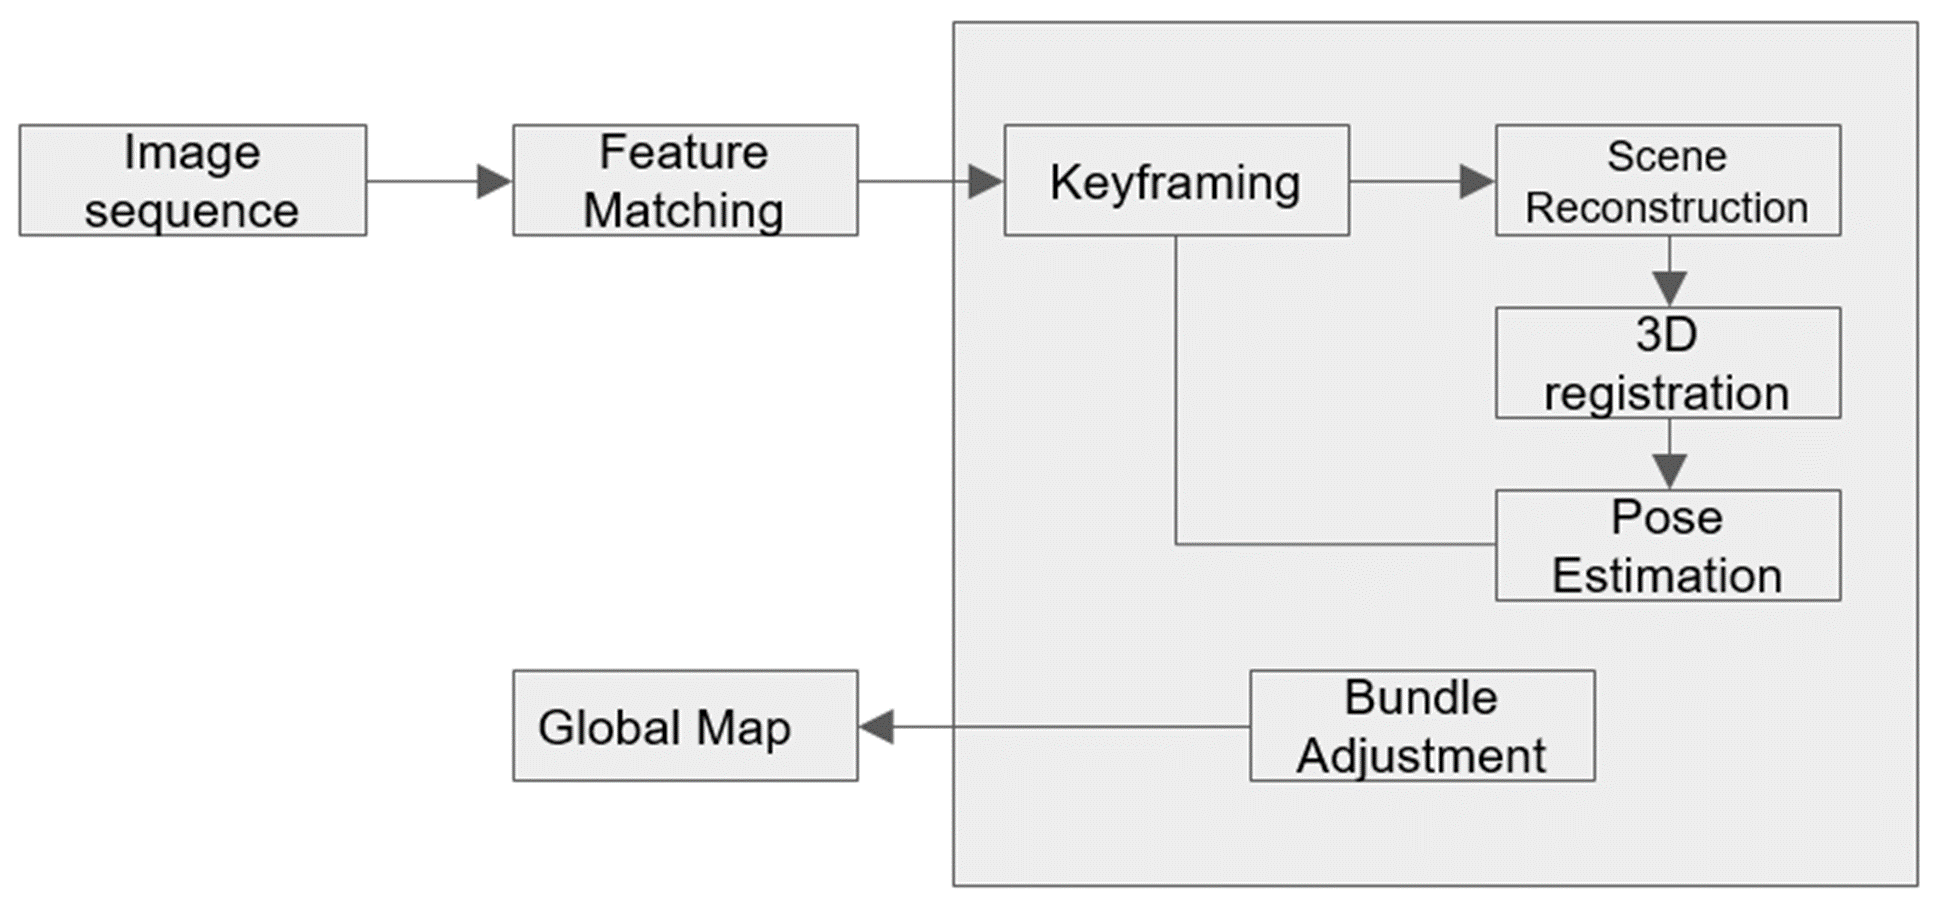
\includegraphics[width=\linewidth]{./system.png}
        \caption{}
        \label{fig:system}
    \end{subfigure}
    \begin{subfigure}[b]{.29\linewidth}
        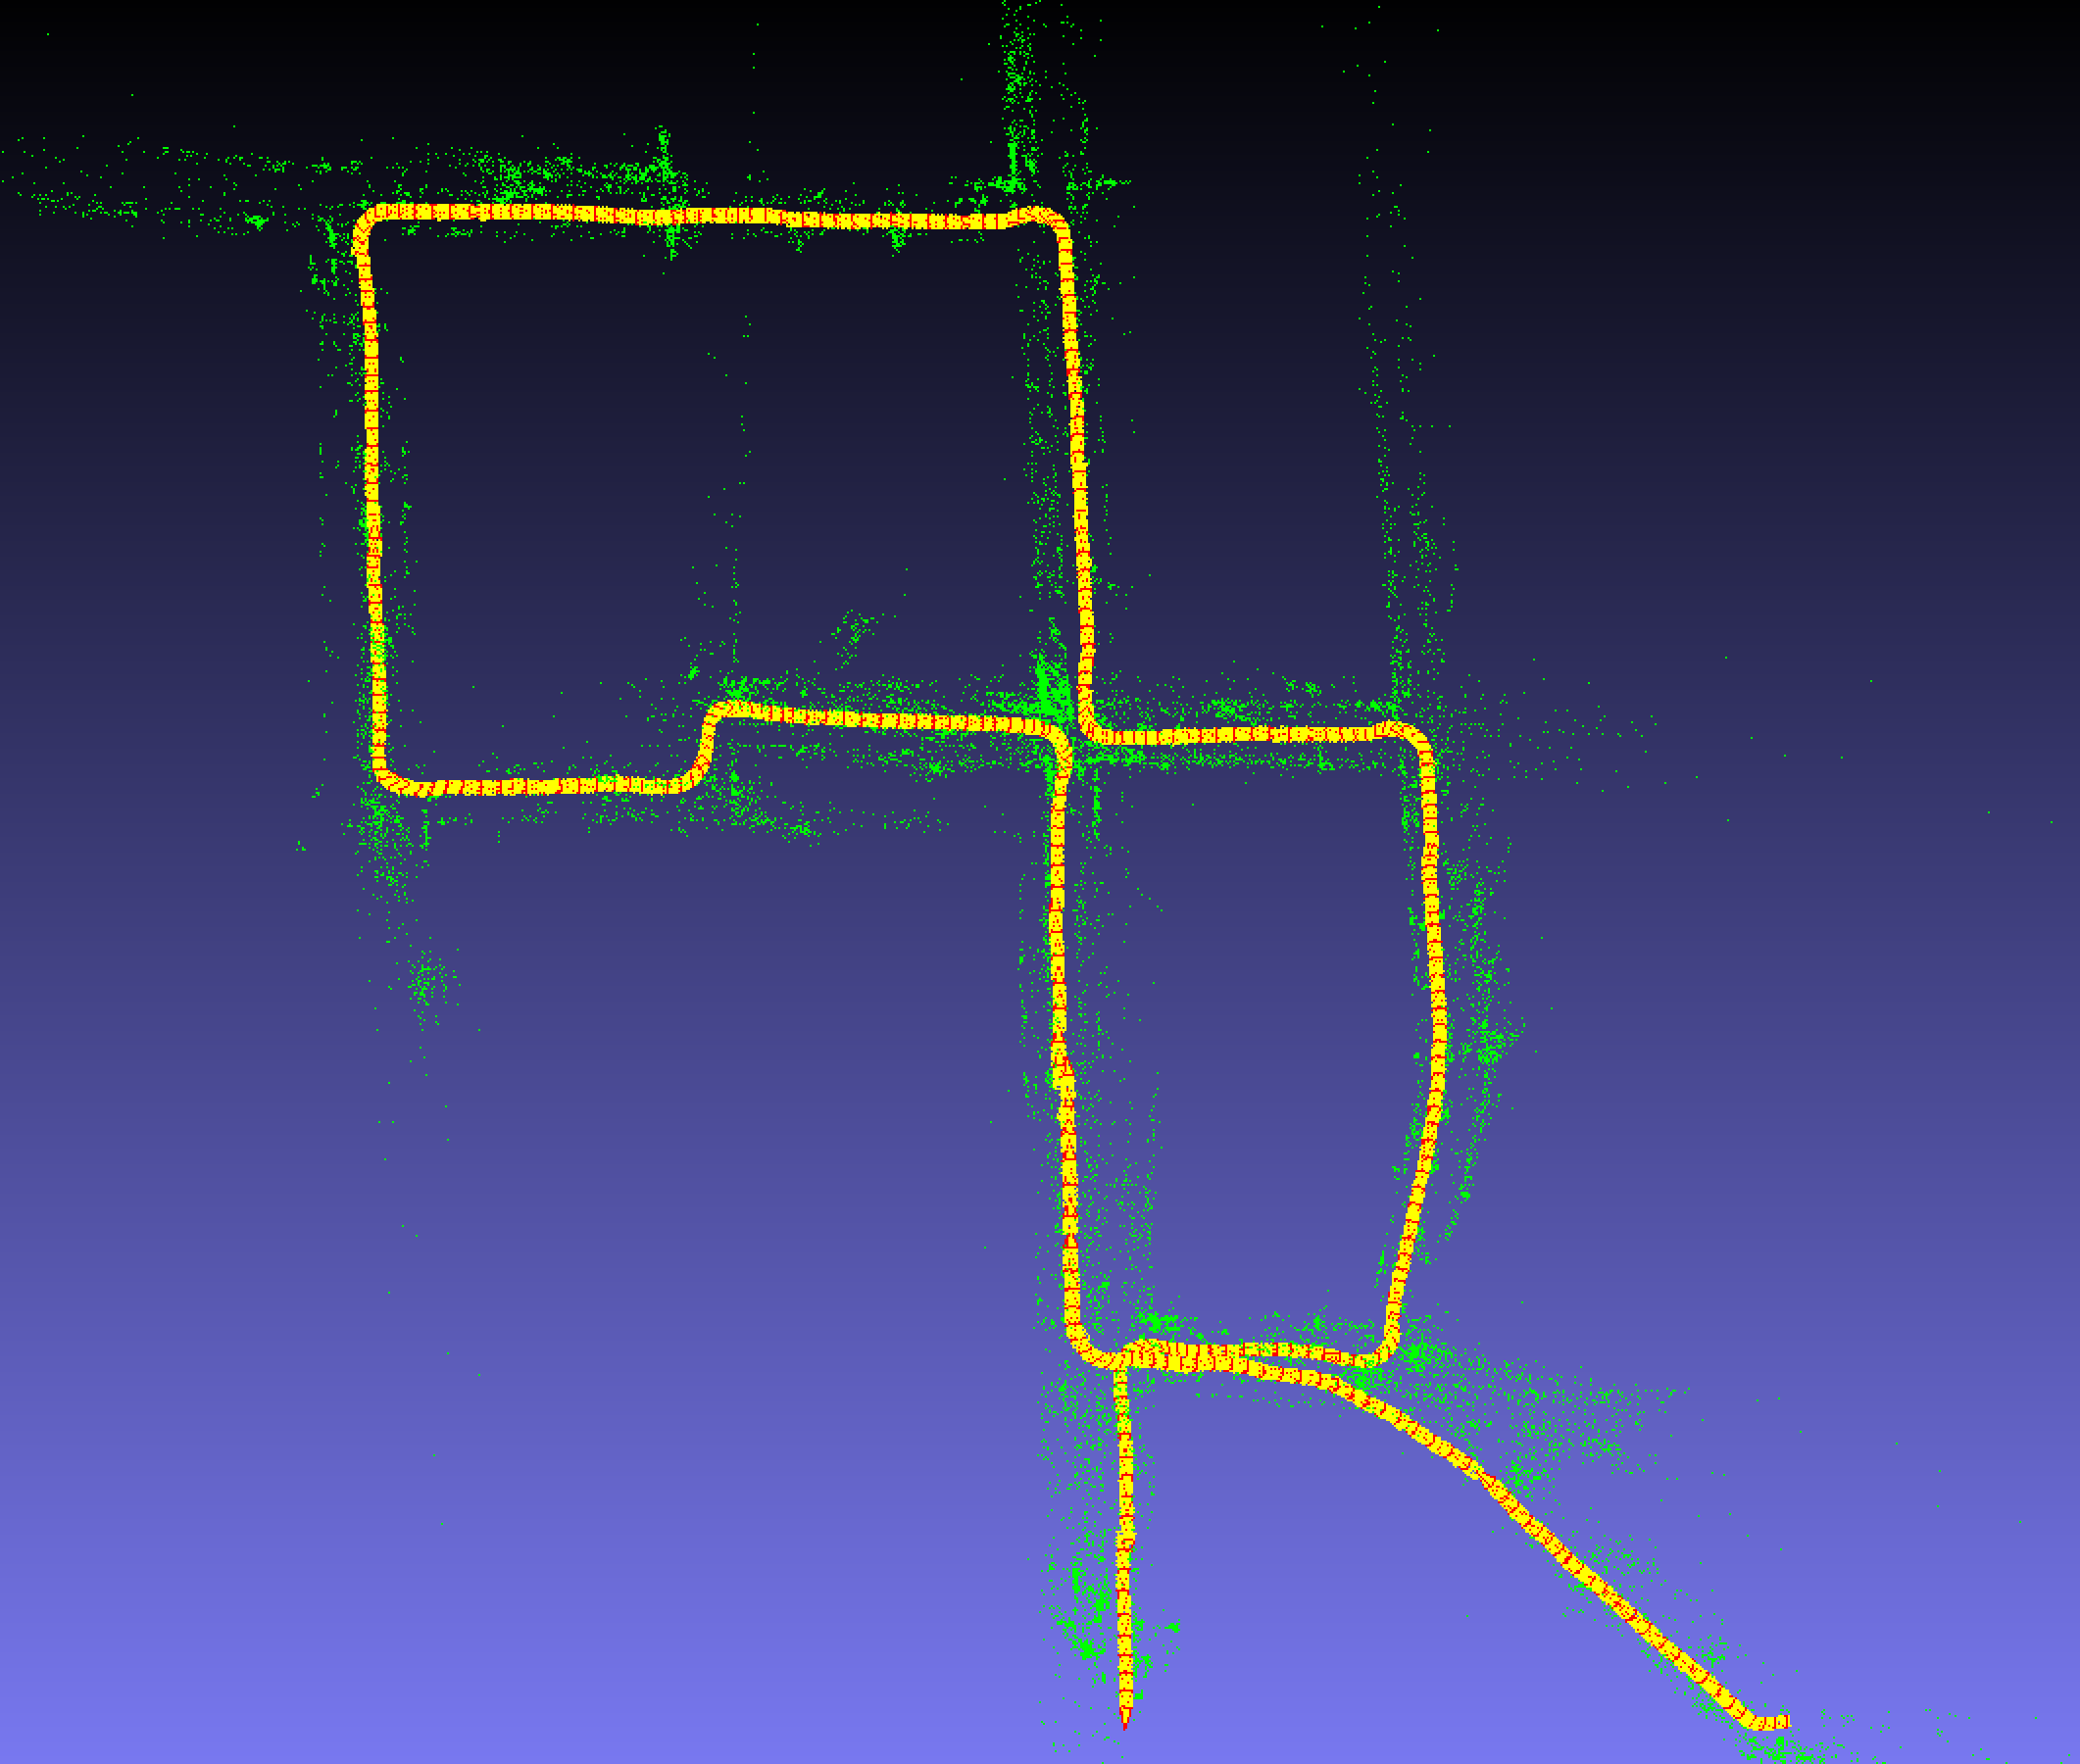
\includegraphics[width=\linewidth]{./vo_stereo_5.png}
        \caption{}
        \label{fig:firstresult}
    \end{subfigure}
    \caption{(a) Overall system architecture. Boxes on the right are what we implemented in this project (b) Results from visual odometry on one of the datasets.}
\end{figure}

\section{System}
Our overall system consists of multiple algorithms as described in Figure \ref{fig:system}. We developed most of the algorithms from scratch and experimented and found the best parameters for each block in the system diagram. Our implementation uses OpenCV\cite{opencv} for computer vision tasks and Ceres solver\cite{ceres-solver} for the non-linear optimization.

\begin{itemize}
\item We take a sequence of images and find good feature matches between two frames.
\item Each frame is tested against few heuristics to decide if it is a keyframe or not.
\item Once keyframes are obtained, then we reconstruct the scene using the key-frames.
\item The poses of the intermediate frames (not the key-frames) are found using PnP algorithm.
\item Bundle adjustment is then performed using data from last m frames.
\end{itemize}

We discuss each of the methods in details in the following sections.

\subsection{Feature Extraction and Matching}
We have experimented with KLT features, AKAZE features and ORB features. The KLT features can also be used for tracking the features in the subsequent frames using optical flow. For AKAZE\cite{akaze} and ORB features, the correspondences are found using feature matching. Experimentally, we found that AKAZE was able to generate good matches and in greater number than the other two approaches for the KITTI datasets\cite{kitti}.

To remove outliers from the matches, we use three tests. The first is the \textbf{ratio test} which ensures that the feature is discriminative enough. This is accomplished by calculating the ratio of the distances between the best match and the second best match for a feature. A discriminative feature would have a high ratio and thus be a good feature to keep.

The second test is the \textbf{symmetry test} where we ensure that matches from image $\textbf{I}_i$ to $\textbf{I}_j$ also match in the reverse direction - that is from $\textbf{I}_j$ to $\textbf{I}_i$. The third test is the \textbf{epipolar test} where we discard matches that do not satisfy the epipolar geometry of the two frames used for 3D reconstruction. Using these three criteria we get rid of the most of the outliers in feature matching. An example of feature matches is shown in Figure \ref{fig:matches}.

\begin{figure}
    \centering
    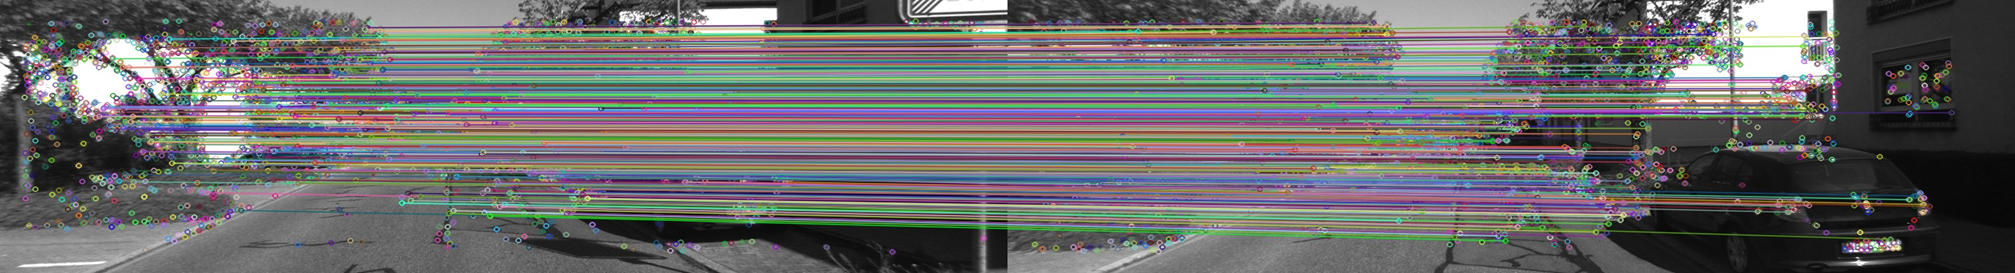
\includegraphics[width=\linewidth]{./matches.png}
    \caption{An example of feature matches between two consecutive fraames of the KITTI dataset. These are results after all outliers have be removed.}
    \label{fig:matches}
\end{figure}

\subsection{Keyframing}

\begin{figure}
\centering
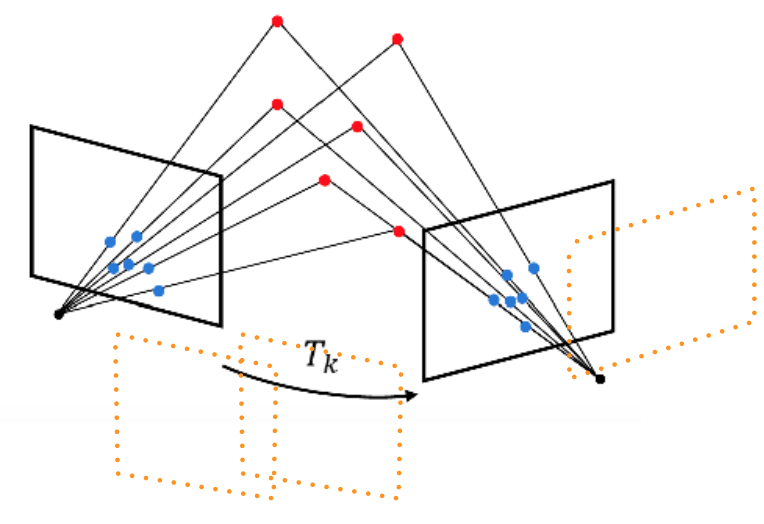
\includegraphics[width=0.5\textwidth]{./system_viz}
\caption{Vizualization of the keyframes and the intermediate frames. The keyframes are used for 3D reconstruction and the pose of the intermediate frames are found using Perpective-n-point algorithm}
\label{fig:keyframing}
\end{figure}

3D reconstruction is expensive and thus we want to limit it to only a few frames. This is done using keyframing where only specific frames are picked for 3D reconstruction and other frames use the point cloud generated from these frames as shown in the figure \ref{fig:keyframing}.

Our first approach was to have every frame be a keyframe - this is expensive to compute since you need to evaluate the feature matches, triangulate points and also recover pose. Our second approach was to have every 5th frame be a keyframe. This approach worked very well for motion along a straight line but drifted significantly when the camera turned. Our third approach and current approach is based on the number of feature matches between the current and previous keyframe. If the count is below a certain threshold (45\% in our case), then we trigger creating a new keyframe and the corresponding 3D reconstruction.

Another approach we considered was using a homography based test\cite{homography}. However, we found that the feature match count approach worked better for our dataset.

\subsection{3D scene reconstruction}
Using the feature matching, we can find the fundamental matrix. The fundamental matrix gives the relationship between the feature points. We use a RANSAC based 5-point algorithm to find the fundamental matrix.

Using this fundamental matrix, we can estimate the camera pose between the two images. However, this gives rise to four possible camera configurations (with $W$/$W^T$ and $\pm t$) as described in \cite{Hartley2004}. The correct location can be found using the camera configuration in which all the points are in front of both the cameras.

The triangulation can be done in two modes: one with stereo image pairs and one with a monocular images. Once a frame is labelled as a keyframe, we generate the reconstruction of the scene either by using the stereo pair or reconstruction using the previous keyframe in monocular case. Reconstruction in both modes was successful. However, as hypothesized, we noticed qualititively that the monocular 3D reconstruction had more drift compared to the stereo reconstruction.

\begin{figure}
    \centering
    \begin{subfigure}[b]{.45\linewidth}
        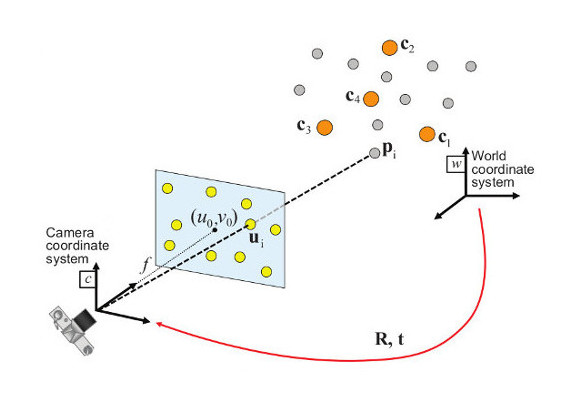
\includegraphics[width=\linewidth]{./pnp.jpg}
        \caption{}
        \label{fig:pnp}
    \end{subfigure}
    \begin{subfigure}[b]{.45\linewidth}
        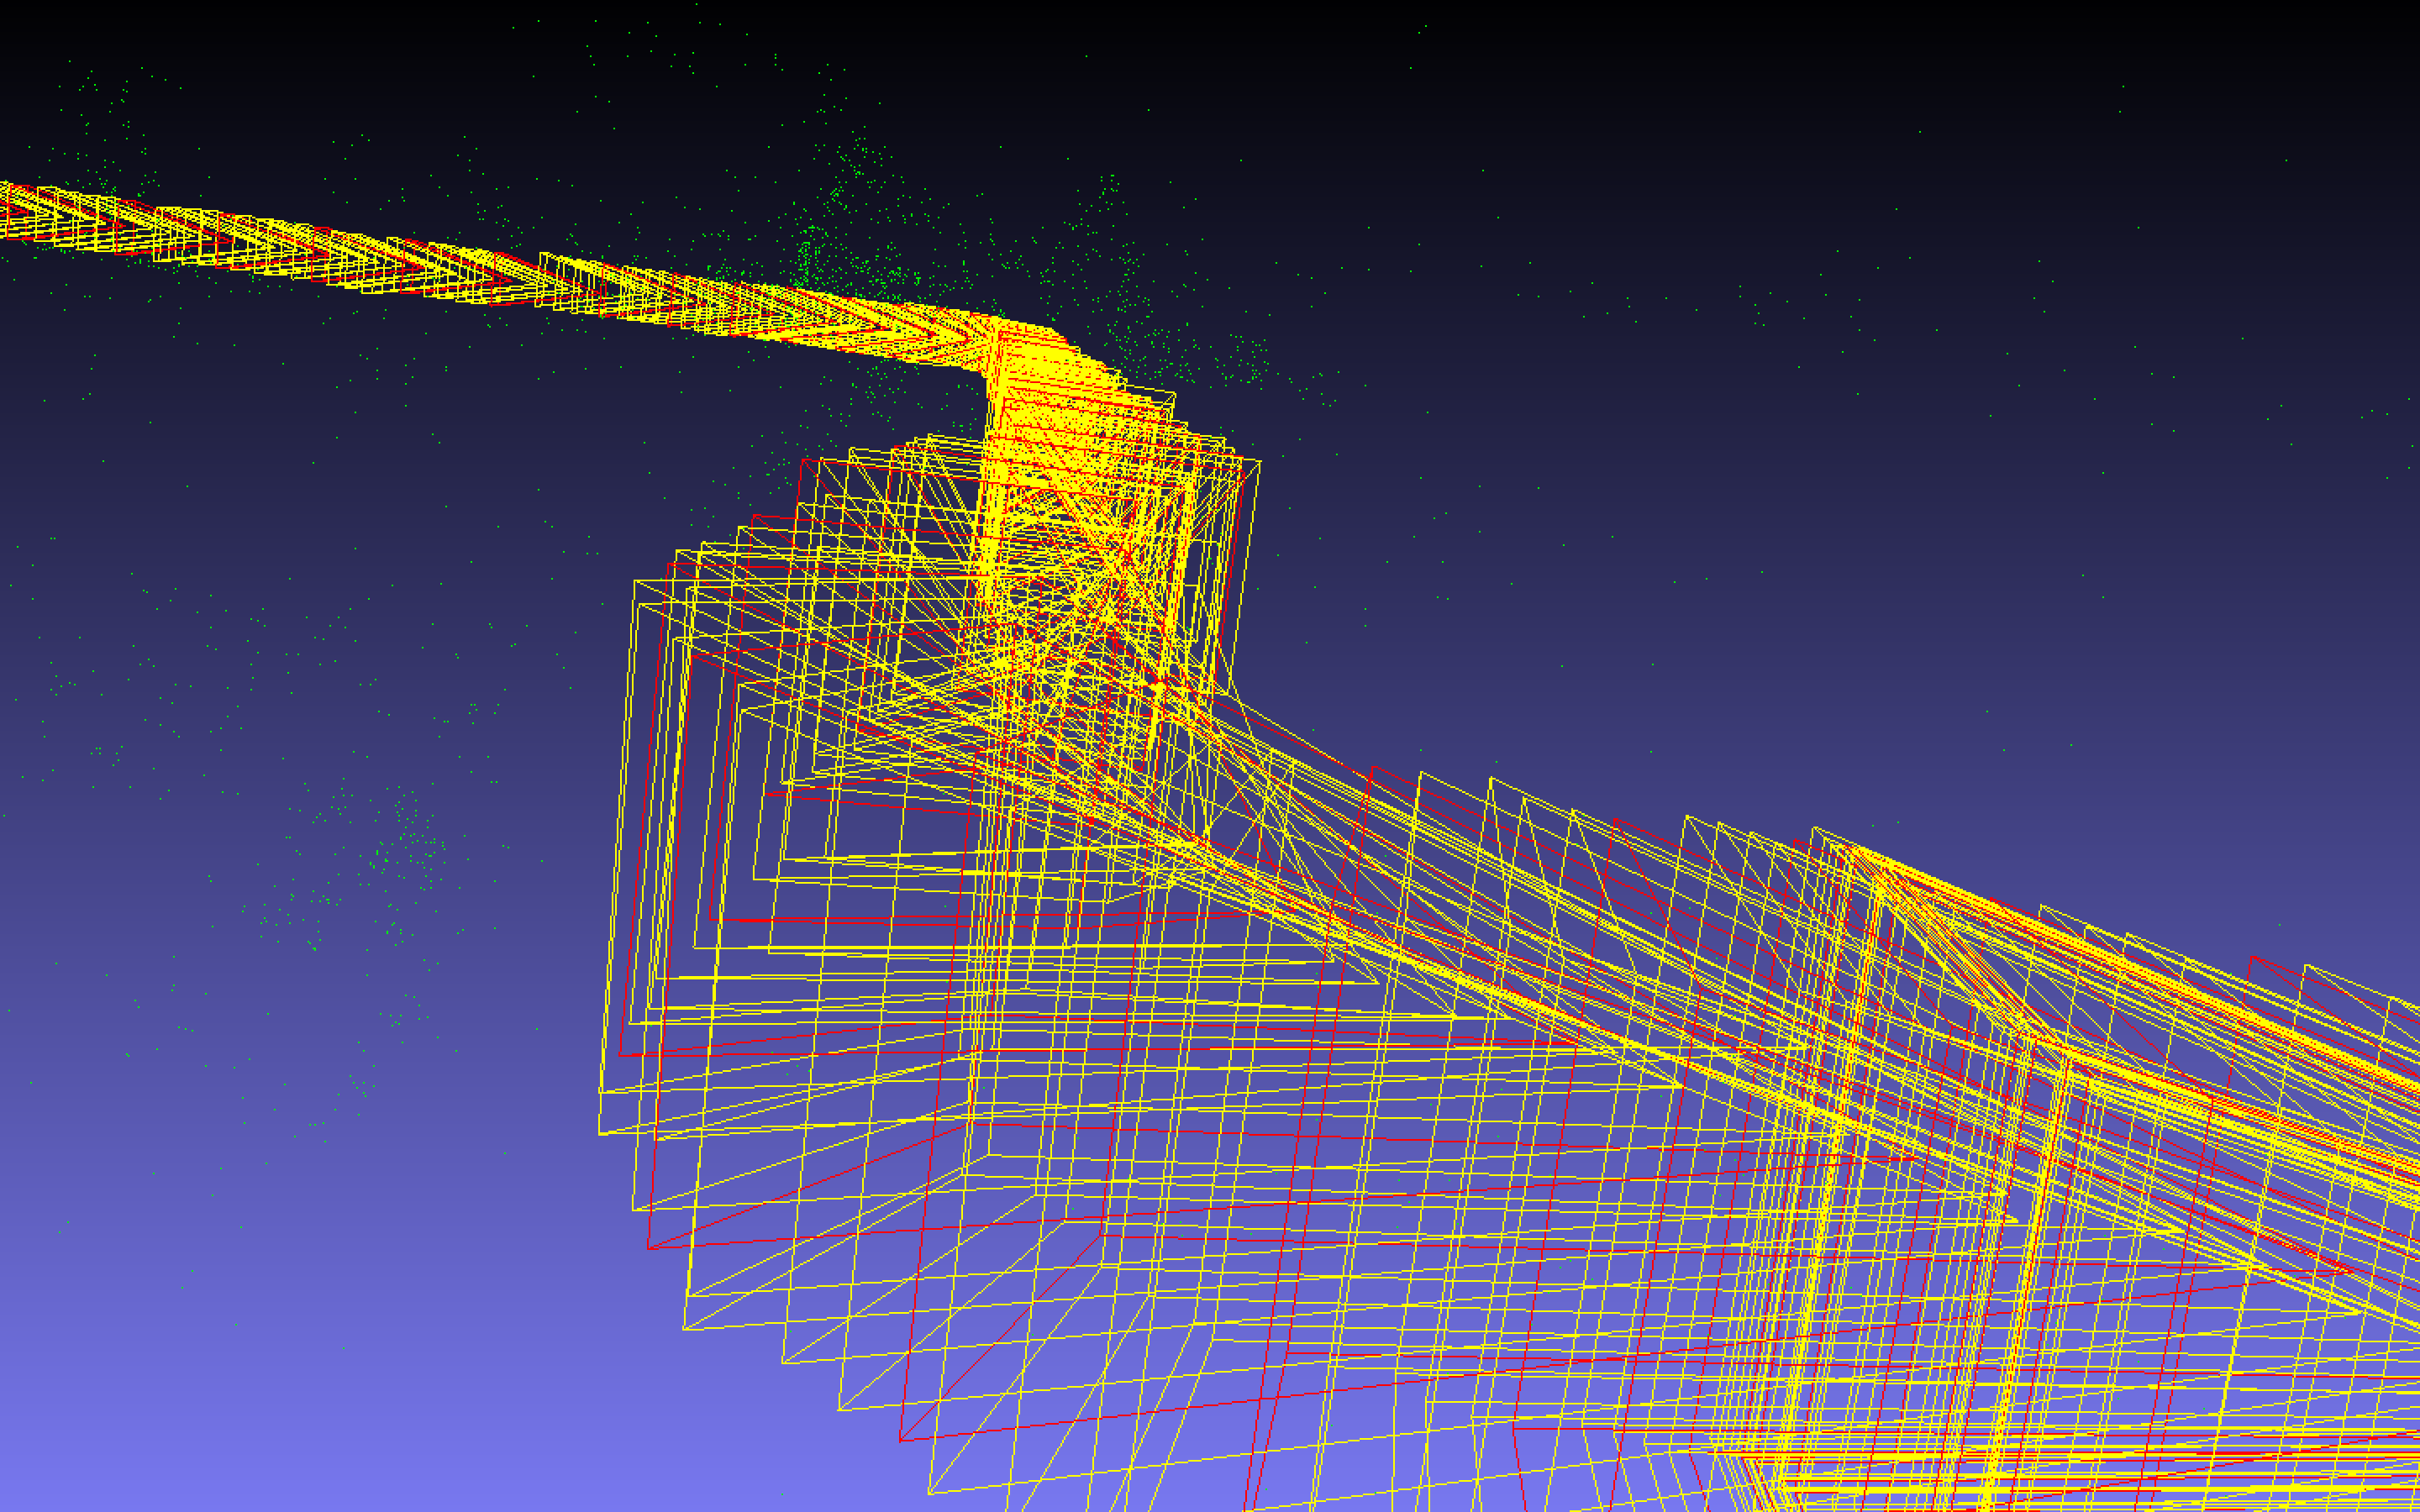
\includegraphics[width=\linewidth]{./vo_stereo_7.png}
        \caption{}
        \label{fig:recon}
    \end{subfigure}
    \caption{(a) Using PNP to estimate the camera pose using the global 3D point cloud and the corresponding observations in the image. (b) Three dimensional reconstruction (points in green) and the camera poses corresponding to them}
\end{figure}

\subsection{Point cloud registration}
As an image sequence proceeds, we use the current keyframe and the previous keyframe (or the current keyframe and the corresponding right-eye image in case of stereo) to reconstruct a point cloud based on feature matches. However, the point clouds might be of a different scale and would need to be registered to a global coordinate system.

One approach to calculate the scale of the point cloud is to fit gaussian to the scaling factors obtained by pairwise distances between 3D points in two point clouds. Using the mean of the distances in the local pointcloud and the global pointcloud, we can calculate the scale. Once we have the scale, we can compute the rotation and translation of the point cloud using the common feature points.

To compute the rotation and translation, we use the method described in \citep{rigid}

\begin{align*}
    (\textbf{R}, \textbf{t}) &= \min_{\textbf{R} \in SO(3), \textbf{t} \in \mathbb{R}^{3}} \sum_i || \textbf{Rp}_i + \textbf{t} - \textbf{q}_i||^{2}_{2}\\
    \tilde{\textbf{p}} &= \frac{1}{n} \sum_i^{n} \textbf{p}_i\\
    \tilde{\textbf{q}} &= \frac{1}{n} \sum_i^{n} \textbf{q}_i\\
    \textbf{x}_i &= \textbf{p}_i - \tilde{\textbf{p}_i}\\
    \textbf{y}_i &= \textbf{q}_i - \tilde{\textbf{q}_i}\\
    \textbf{S} &= \textbf{XWY}^{T} = \textbf{U}\Sigma\textbf{V}^{T} & \text{(SVD)}\\
    \textbf{R} &= \textbf{V} \begin{bmatrix}
        1 & \cdots & \cdots\\
        \cdots & 1 & \cdots\\
        \cdots & \cdots & \det(\textbf{VU}^{T})\\
    \end{bmatrix} \textbf{U}^{T}\\
    \textbf{t} &= \tilde{\textbf{q}} - \textbf{R}\tilde{\textbf{p}}\\
\end{align*}

Here, \textbf{X} is a $3\times n$ matrix with $\textbf{x}_i$ as columns. \textbf{Y} is defined similarly. \textbf{W} is the weighting matrix - which is identity in our case.

Another approach is to ensure that all projection matrices and transformations occur in one global frame of reference. We assume the first keyframe to be at the origin and chain transformations together to get the current pose.

\subsection{Camera pose recovery}
Once the scene is reconstructed using the keyframes, the camera pose for normal frames can be recovered using Perspective-n-point (PnP) algorithms. By knowing the 3D points from the reconstruction, and its corresponding feature location in any image the camera pose can be recovered using PnP, as shown in Figure \ref{fig:pnp}.

We chain these camera poses together to produce an initial guess of the camera trajectory. The trajectory from such chaining drifts as the sequence proceeds and errors accumulate. To account for these errors in the camera projection matrix (and also the point cloud reconstruction), we use bundle adjustment over the past m frames.

The rotation and the translation obtained from the PnP algorithm in OpenCV gives the tranformation of the camera with respect to the camera frame of reference. To obtain the motion of the camera with respect to global frame of reference, we can just do the inverse.

$$ \textbf{T}_{camera}  = \begin{bmatrix}
\textbf{R}_{3\times3} & \textbf{t} \\
\textbf{0}_{1\times3} & 1
\end{bmatrix} $$

$$ \textbf{T}_{world}  = \begin{bmatrix}
\textbf{R}^T  & -\textbf{R}^T \textbf{t}\\
\textbf{0}_{1\times3} & 1
\end{bmatrix} $$


An illustration of the camera pose recovery is shown in the figure \ref{fig:camerapose}. The green point shows the reconstruction using the keyframe and the intermedite camera pose is obtained using PnP.

\begin{figure}
    \centering
    \begin{subfigure}[b]{.45\linewidth}
        \centering
        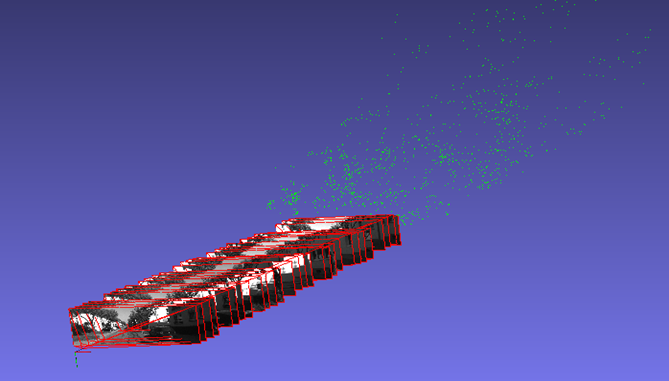
\includegraphics[width=\linewidth]{./camera-pose.png}
        \caption{}
        \label{fig:camerapose}
    \end{subfigure}
    \begin{subfigure}[b]{.45\linewidth}
        \centering
        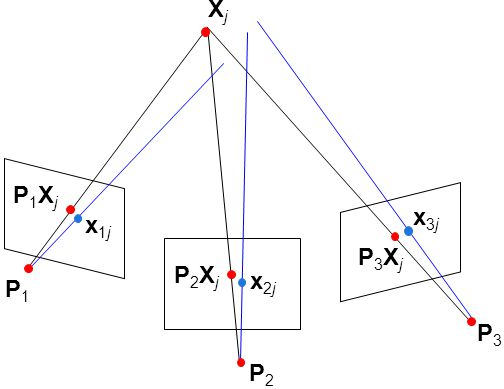
\includegraphics[width=.7\linewidth]{./bundle-adjustment.png}
        \caption{}
        \label{fig:ba}
    \end{subfigure}
    \caption{(a) Recovering camera pose from the point cloud (b) Visualizing bundle adjustment}
\end{figure}

\subsection{Bundle Adjustment}
In visual odometry, the current camera pose is obtained by adding the last observed motion to the current detection change. This leads to a superlinear increase in pose error over time. In this section, we look at the techniques we use to correct this pose drift.

Bundle adjustment can be used to impose geometrical constraints over multiple frames as shown in Figure \ref{fig:ba}. The computational cost increases with the cube of the number of frames used for computation. Thus, we limit the number of frames to a small window from the previously captured frames. This approach is called local bundle adjustment.

We use a local bundle adjustment that affects the global point cloud and the recent m camera poses. We track visibility of 3D points in each frame and use that to construct a cost function. 

\begin{align*}
    &\min_{\textbf{M}_i, \textbf{X}_j} \sum_{i=0}^{m} \sum_j || \textbf{x}^{i}_{j} - \textbf{M}^{i} \textbf{X}_j||^{2}_{2}
\end{align*}

For the camera projection matrices $\textbf{M}^{i}$, we assume that the intrinsics are known and constant. We optimize over the space of all $3 \times 4$ matrices and it converges in about 100 iterations.

After accounting for visibility of keypoints, our optimization has about fifteen thousand variables for $m = 10$. This number depends on the type of image features used (ORB, AKAZE, etc). We use the dense schur method for optimization and use Ceres solver\cite{ceres-solver}. The optimization is able to reduce reprojection error across multiple frames as shown in Figure \ref{fig:reproj}.

\begin{figure}
    \centering
    \begin{subfigure}[b]{.45\textwidth}
        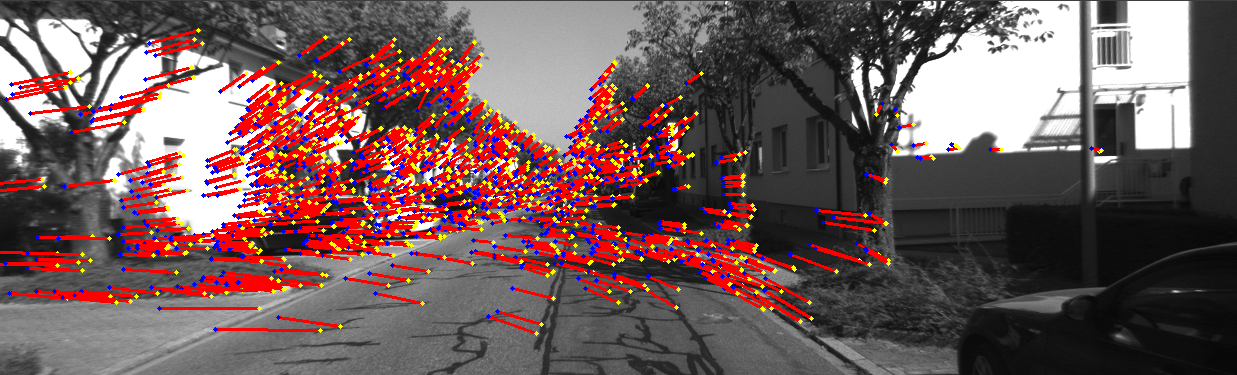
\includegraphics[width=\linewidth]{./before-ba.png}
        \caption{}
    \end{subfigure}
    \begin{subfigure}[b]{.45\textwidth}
        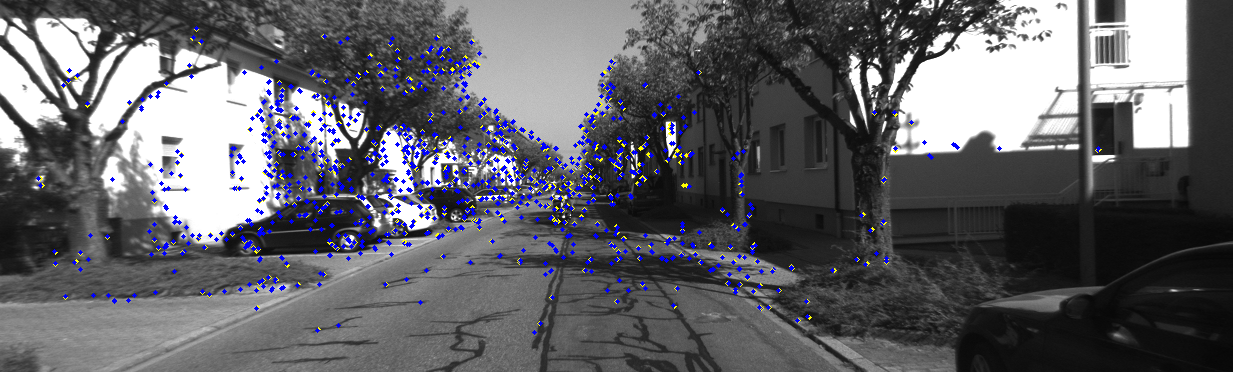
\includegraphics[width=\linewidth]{./after-ba.png}
        \caption{}
    \end{subfigure}
    \caption{(a) Before bundle adjustment, the red lines show the reprojection error between observed keypoints (yellow) and reprojected points (blue). (b) After bundle adjustment, all reprojected points align very closely to the observed feature points}
    \label{fig:reproj}
\end{figure}

\section{Results}
After implementing the above algorithms we were able to get a good localization of the camera on the KITTI datasets \citep{kitti}. The methods are eveluated against the ground truth qualitatively. The results are shown for the stereo, monocular and monocular with bundle-adjustment.

\subsection{Stereo visual odometry}
In steroscopic visual odometry, we used a stereo pair at every keyframe. The baseline between the stereo pair was about \textbf{0.54m} and this helped produce very accurate visual odometry. The reconstruction using the stereo pair is shown in the figure \ref{fig:reconstruction}. The stero reconstruction is better than the monocular reconstrctuction.

\begin{figure}
\begin{subfigure}{0.5\textwidth}
\centering
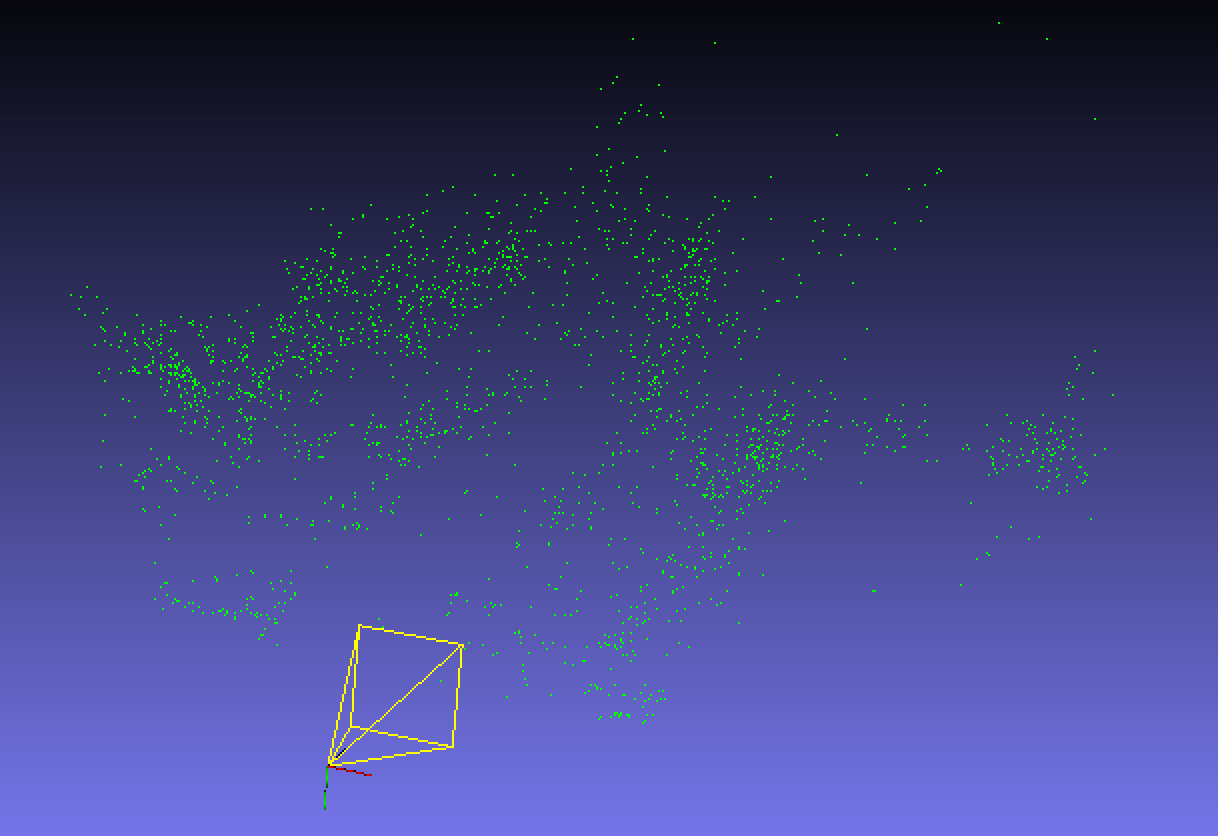
\includegraphics[height=0.5\textwidth]{./mono_reconstruction}
\end{subfigure}
\begin{subfigure}{0.5\textwidth}
\centering
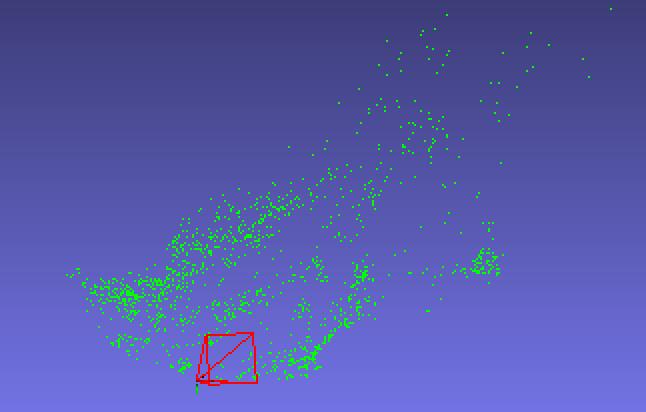
\includegraphics[height=0.5\textwidth]{./stereo_reconstruction}
\end{subfigure}
\caption{(a) Monocular 3D reconstruction and (b) Stereo 3D reconstruction}
\label{fig:reconstruction}
\end{figure}


We used this experiment as a baseline to test how good the monocular visual odometry is.

\begin{figure}[h]
    \centering
    \begin{subfigure}[b]{.45\textwidth}
    \centering
        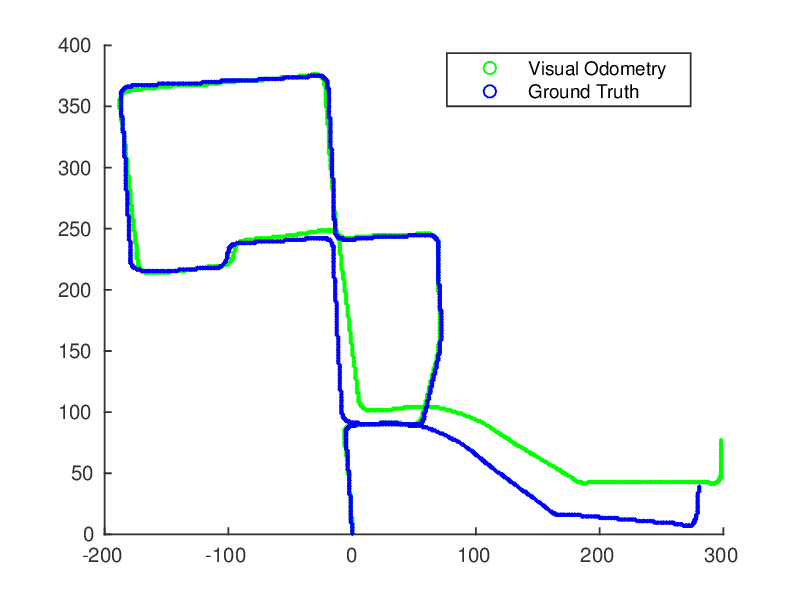
\includegraphics[width=\linewidth]{./avisingh}
        \caption{}
    \end{subfigure}
    \begin{subfigure}[b]{.45\textwidth}
    \centering
        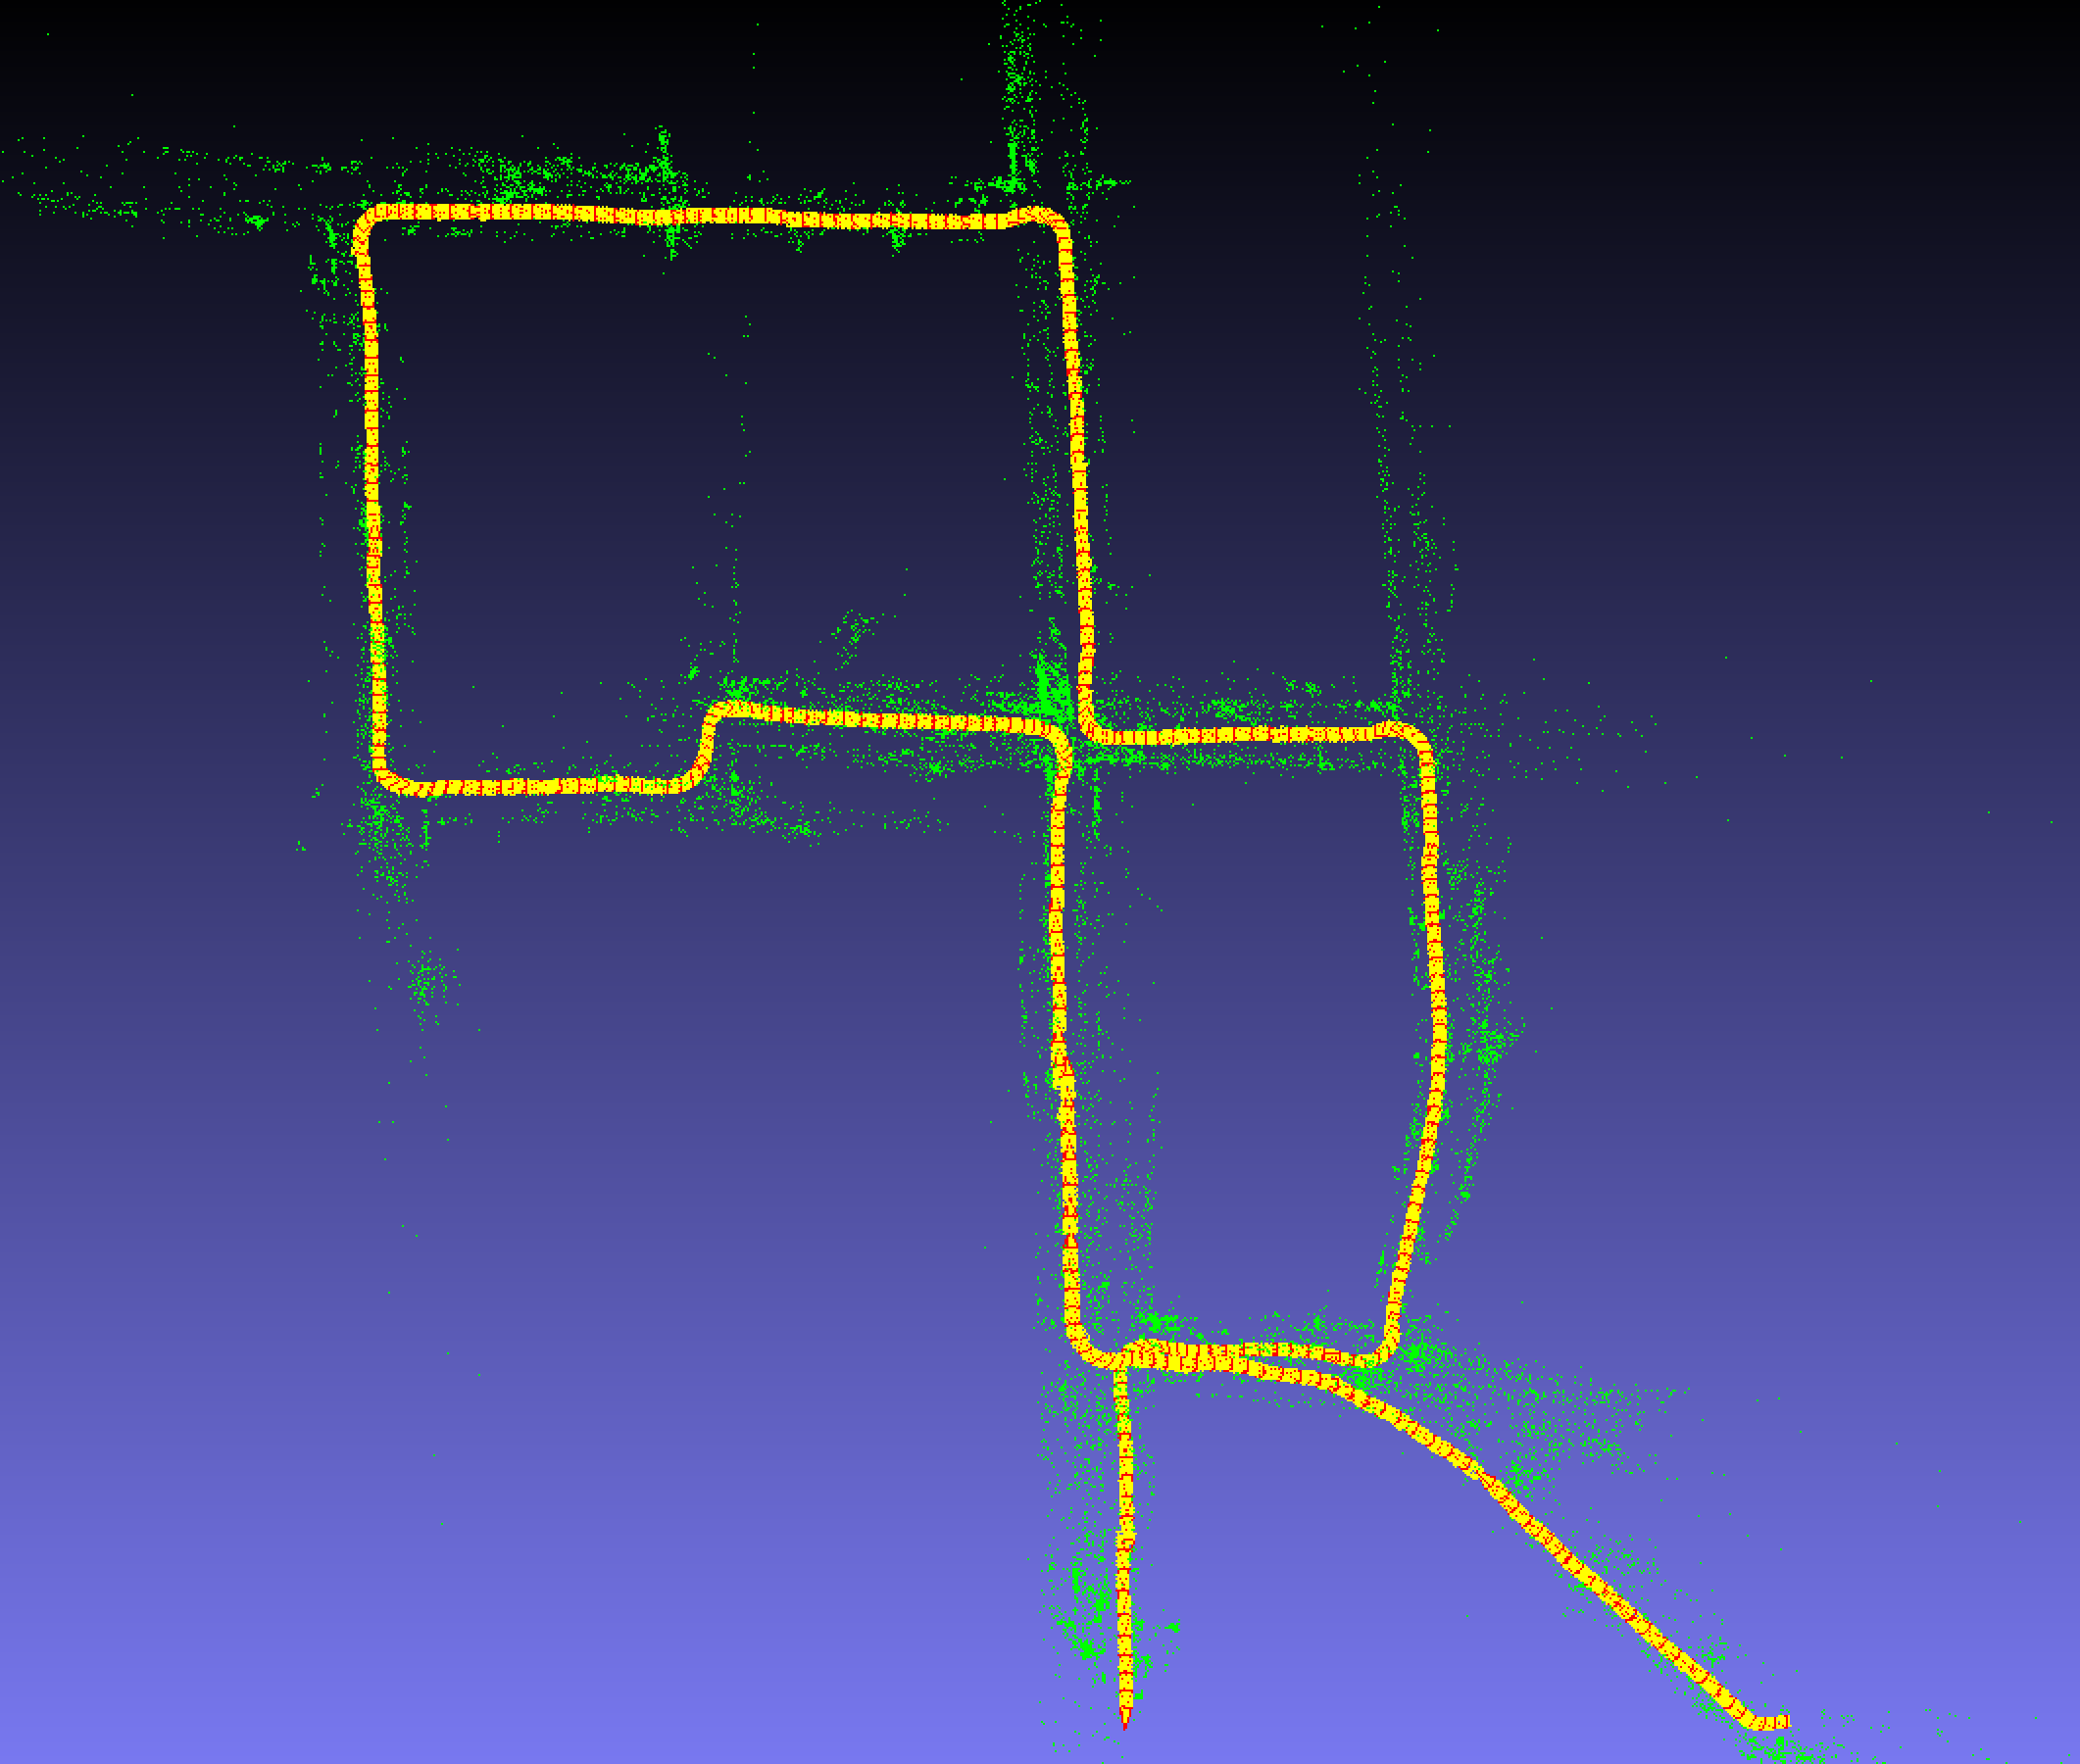
\includegraphics[width=\linewidth]{./vo_stereo_5}
        \caption{}
    \end{subfigure}
    \caption{Evaluation of our stereo visual odometry against ground truth. (a) The ground-truth trajectory with a baseline implementation. (b) Our stereo Visual Odometry implementation.}
    \label{fig:groundtruth}
\end{figure} 

   
\begin{figure}    
    \begin{subfigure}[b]{.45\textwidth}
    \centering
        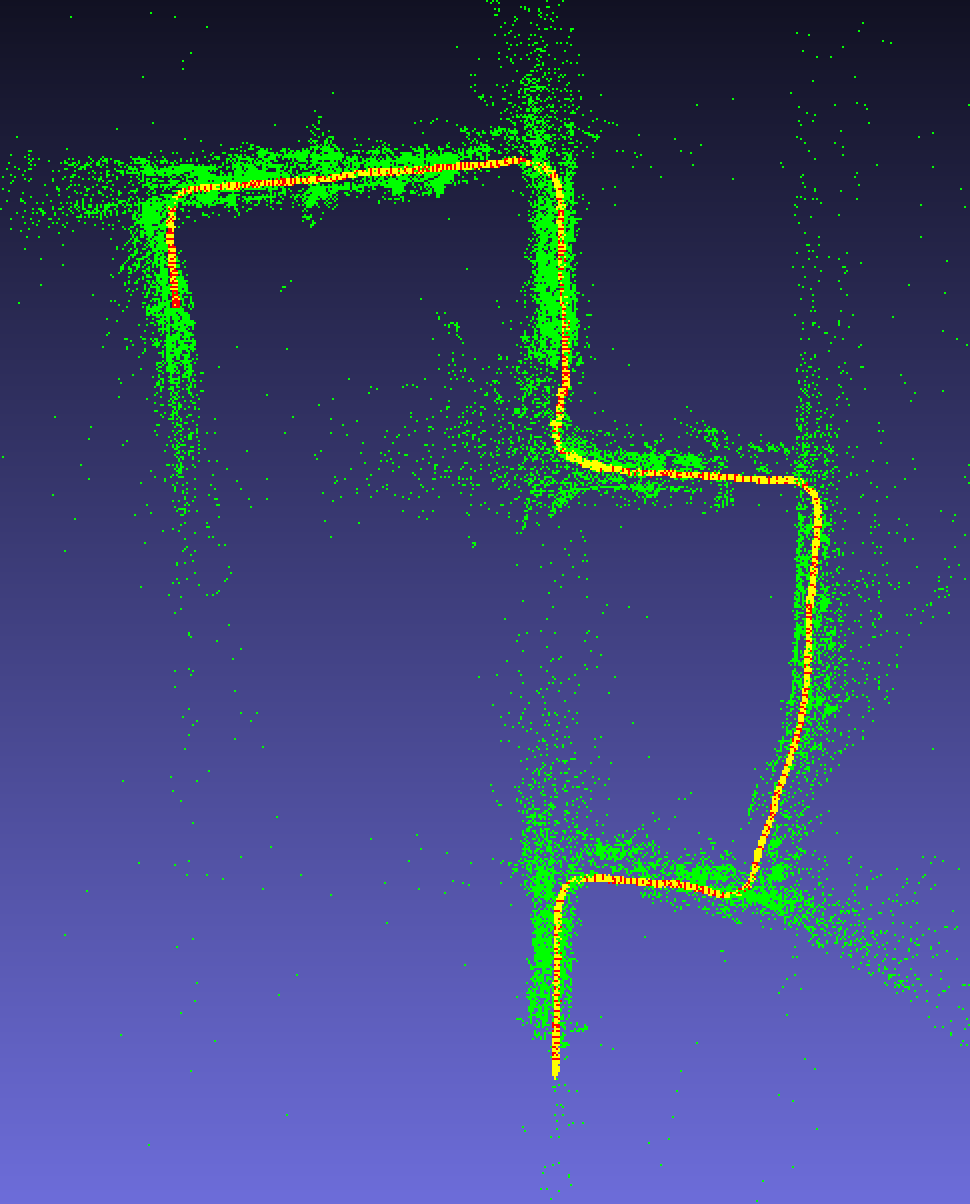
\includegraphics[height=0.7\linewidth]{./vo_mono_3.png}
        \caption{}
        \label{fig:mono}
    \end{subfigure}
    \begin{subfigure}[b]{.45\textwidth}
    \centering
        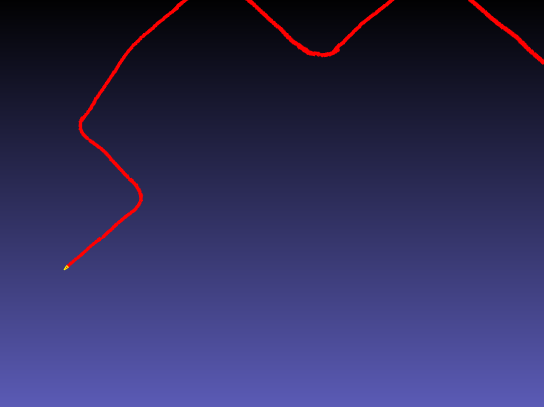
\includegraphics[height=0.7\linewidth]{./mono-ba.png}
        \caption{}
        \label{fig:monoba}
    \end{subfigure}
    \caption{Monocular Visual odometry (a) Using only monocular image pairs (b) Using monocular image pairs and bundle adjustment.}
\end{figure}

\begin{figure}
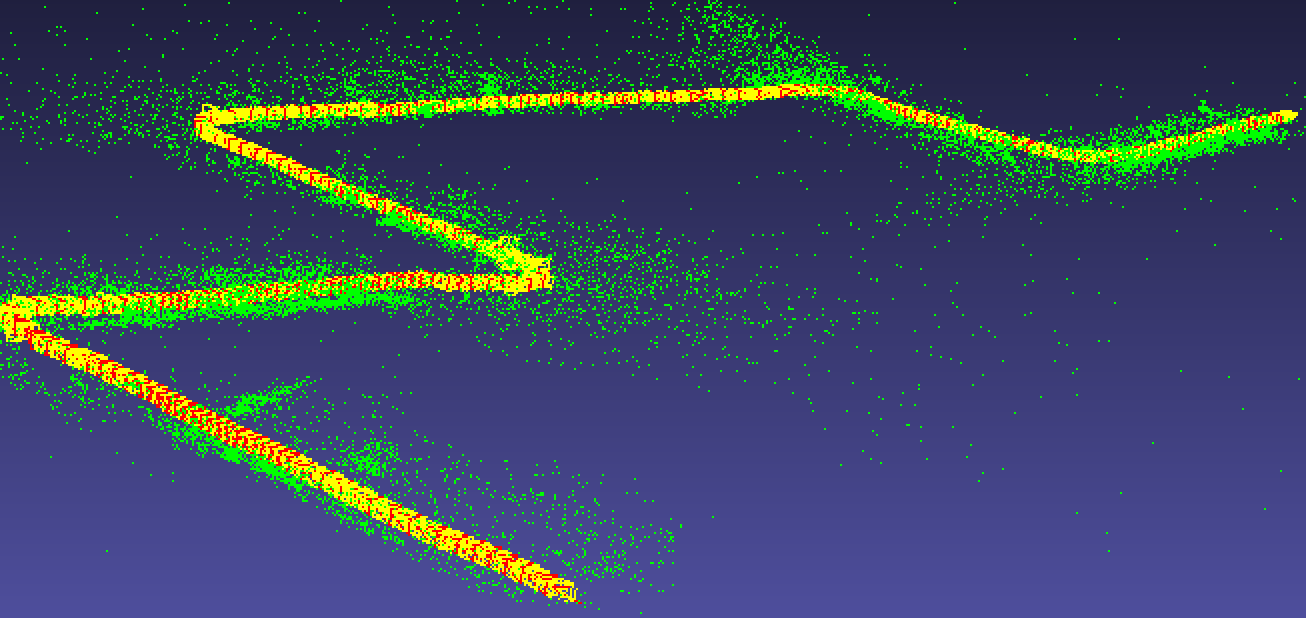
\includegraphics[width=\textwidth]{./path}
\caption{Visualization of monocular visual odometry along with its path. The green dots are the landmarks in the scene and the red frustum are the keyframe locations and the yellow camera frustrums are the intermediate frames}
\label{fig:closeup}
\end{figure}

\subsection{Monocular visual odometry}
With the monocular case, we used the previous keyframe's image instead of the right eye of the stereo pair. Doing this required writing special code to get the system initialized (the first keyframe would have no 3D reconstruction associated with it). However, once initialized, the system works well and produces the familar trajectory.

\subsection{Monocular visual odometry with bundle adjustment}
To improve results for the monocular visual odometry, we enabled bundle adjustment and executed it on the same datasets as in previous experiments. We found that the results were better qualitatively and produce a good trajectory of the camera as seen in Figure \ref{fig:monoba}.

However, the code execution speed slowed down quite a bit. We found that an optimization over the past 10 frames requires about fifteen thousand variables and takes several milliseconds to execute. We currently optimize over the extrinsic matrix and assume that the intrinsics are known and correct. Our hypothesis is that optimizing over the SE(3) manifold would help converge the optimization in fewer iterations and potentially to a better solution as well. This is because it would enforce the rotation matrix to be orthonormal.


\section{Future Work}

Currently, we calculate the fundamental matrix using the Ransac version of the 5-point algorithm. However, it is possible to improve upon this by using the three-point algorithm\cite{threepoint}. This requires integration with the IMU as an additional clue for estimating the fundamental matrix.

Another area to improve is selecting when to generate a new keyframe. We use the number of keyframe feature matches as the selection criteria. A more mathematically grounded technique would be to use the covariance of the various points to do this.

Our data structures used for storing point correspondences, the 3D point cloud, etc can be made much more memory and complexity efficient. While this wouldn't contribute to computer vision, it would allow us to run experiments faster and better tune the algorithm to be more generic.

Finally, we hope to model the point cloud as probability densities or planes. This would reduce the memory footprint and potentially improve the quality of pose estimation.

\section{Conclusion}
We implemented an end-to-end pipeline for visual odometry and included key concepts like keyframing, monocular 3D reconstruction, point cloud registration, camera pose recovery and bundle adjustment. We experimented with multiple configurations - stereo, monocular and monocular plus bundle adjustment.

Our system can take a dataset as an input and produce a motion trajectory of the camera. We hope to use this system in the future, improve upon it and use it as a starting point for future research.

\bibliographystyle{unsrt}
\bibliography{nips_2016}

\begin{comment}
\begin{thebibliography}{15}

\bibitem{vo}
Nister

\bibitem{akaze}

      \bibitem{akaze} P. Alcantarilla, J. Nuevo and A. Bartoli, \textit{Fast Explicit Diffusion for Accelerated Features in Nonlinear Scale Spaces}, BMVC 2013
      \bibitem{threepoint} F. Fraundorfer, P. Tanskanen and M. Pollefeys \textit{A minimal case solution to the calibrated relative pose problem for the case of two known orientation angles}, ECCV 2010.
       \bibitem{vo} D. Nister, O. Naroditsky and J. Bergen \textit{Visual Odometry}, CVPR 2004
       
       \bibitem{homography} O. D. Faugeras and F. Lustman, \textit{Motion and structure from motion in a piecewise planar environment}, IJPRAI, 1988

       \bibitem{semidense} T. Schops, J. Engel and D. Cremers \textit{Semi-Dense visual odometry for AR on a smartphone}
      \bibitem{tumsensor} P. Tiefenbacher, T. Schulze and G. Rigoll \textit{Off-the-shelf sensor integration for mono-SLAM on Smart Devices}, CVPR 2015
      \end{thebibliography}
\end{comment}

%\endgroup

\end{document}
